\documentclass[presentation,aspectratio=43,10pt]{beamer}

\usepackage{mathtools}
\usepackage{hyperref}
\newcommand{\arxivlink}[2]{{\texttt{arXiv:\,\href{https://arxiv.org/abs/#1}{#1\,[#2]}}}}

\titlegraphic{\hfill
\includegraphics[height=1.25cm]{durham-logo}}
\usepackage{appendixnumberbeamer}
\usepackage{amsmath}
\usepackage{amssymb}
\usepackage{minted}

\usepackage[url=false,
doi=true,
isbn=false,
style=authoryear,
maxnames=5,
giveninits=true,
uniquename=init,
backend=biber]{biblatex}
\renewcommand{\bibfont}{\fontsize{7}{7}\selectfont}
\addbibresource{references.bib}

\setlength{\bibitemsep}{1ex}
\setlength{\fboxsep}{1pt}

\renewbibmacro{in:}{}
\DeclareFieldFormat[article]{volume}{\textbf{#1}}
\DeclareFieldFormat{doi}{%
  doi\addcolon%
  {\scriptsize\ifhyperref{\href{http://dx.doi.org/#1}{\nolinkurl{#1}}}
    {\nolinkurl{#1}}}}
\AtEveryBibitem{%
\clearfield{pages}%
\clearfield{issue}%
\clearfield{number}%
}

\DeclareMathOperator{\grad}{grad}
\let\div\relax
\DeclareMathOperator{\div}{div}
\DeclareMathOperator{\curl}{curl}
\DeclareMathOperator{\range}{range}
\usetheme{metropolis}
\setbeamertemplate{title graphic}{
  \vbox to 0pt {
    \vspace*{1em}
    \inserttitlegraphic%
  }%
  \nointerlineskip%
}
\metroset{background=light,progressbar=frametitle,numbering=counter,block=fill}

% https://www.dur.ac.uk/marketingandcommunications/marketing/branding/colourpalette/
% Most of these are indistinguishable to those suffering colour blindness
\definecolor{purple}{HTML}{7e317b}
\definecolor{lightpurple}{HTML}{D8ACE0}
\definecolor{blue}{HTML}{006388}
\definecolor{red}{HTML}{AA2B4A}
\definecolor{green}{HTML}{9FA161}
\definecolor{yellow}{HTML}{E8E391}
\definecolor{pink}{HTML}{C43B8E}
\definecolor{lightblue}{HTML}{C4E5FA}

\setbeamercolor{normal text}{
  fg=black,
  bg=white
}
\setbeamercolor{alerted text}{
  fg=red
}
\setbeamercolor{example text}{
  fg=blue
}

\setbeamercolor{palette primary}{%
  use=normal text,
  fg=normal text.bg,
  bg=purple,
}

\author{Lawrence Mitchell\inst{1,*} \\
  \and {\scriptsize
    P.~E.~Farrell (Oxford)
    \and
    R.~C.~Kirby (Baylor)
    \and
    M.~G.~Knepley (Buffalo)
    \and
    F.~Wechsung (Oxford)}}
\institute{
  \inst{1}Department of Computer Science, Durham University\\
  \inst{*}\texttt{lawrence.mitchell@durham.ac.uk}}

\usepackage{tikz}
\usetikzlibrary{trees,calc,positioning}
\usetikzlibrary{shapes, shapes.geometric}
% https://tex.stackexchange.com/questions/27171/padded-boundary-of-convex-hull
\newcommand{\convexpath}[2]{
  [
  create hullcoords/.code={
    \global\edef\namelist{#1}
    \foreach [count=\counter] \nodename in \namelist {
      \global\edef\numberofnodes{\counter}
      \coordinate (hullcoord\counter) at (\nodename);
    }
    \coordinate (hullcoord0) at (hullcoord\numberofnodes);
    \pgfmathtruncatemacro\lastnumber{\numberofnodes+1}
    \coordinate (hullcoord\lastnumber) at (hullcoord1);
  },
  create hullcoords
  ]
  ($(hullcoord1)!#2!-90:(hullcoord0)$)
  \foreach [
  evaluate=\currentnode as \previousnode using \currentnode-1,
  evaluate=\currentnode as \nextnode using \currentnode+1
  ] \currentnode in {1,...,\numberofnodes} {
    let \p1 = ($(hullcoord\currentnode) - (hullcoord\previousnode)$),
    \n1 = {atan2(\y1,\x1) + 90},
    \p2 = ($(hullcoord\nextnode) - (hullcoord\currentnode)$),
    \n2 = {atan2(\y2,\x2) + 90},
    \n{delta} = {Mod(\n2-\n1,360) - 360}
    in
    {arc [start angle=\n1, delta angle=\n{delta}, radius=#2]}
    -- ($(hullcoord\nextnode)!#2!-90:(hullcoord\currentnode)$)
  }
}

\date{February 27, 2019}
\title{A new configurable preconditioner for subspace correction methods in
  PETSc}

\graphicspath{{./\jobname.figures/}{../pictures/}}

\begin{document}

\maketitle

% \begin{abstract}
%   Small block overlapping, and non-overlapping, Schwarz methods are
%   theoretically highly attractive as multilevel smoothers for a wide
%   variety of problems that are not amenable to point relaxation
%   methods.  Examples include monolithic Vanka smoothers for Stokes,
%   overlapping vertex-patch decompositions for $H(\text{div})$ and
%   $H(\text{curl})$ problems, along with nearly incompressible
%   elasticity and augmented Lagrangian schemes.

%   While it is possible to manually program these different schemes,
%   their use in general purpose libraries has been held back by a lack
%   of generic, composable interfaces.  We present a new approach to the
%   specification and development such additive Schwarz methods in PETSc
%   that cleanly separates the topological space decomposition from the
%   discretisation and assembly of the equations.  Our preconditioner is
%   flexible enough to support overlapping and non-overlapping additive
%   Schwarz methods, and can be used to formulate line, and plane
%   smoothers, Vanka iterations, amongst others.  We illustrate these
%   new features with some examples utilising the Firedrake finite
%   element library.
% \end{abstract}

\begin{frame}
  \frametitle{Some motivating preconditioners}

  \begin{onlyenv}<1>
    \begin{block}{$p$-independent preconditioners for elliptic problems}
      [Each subspace is generated from]
      $V_i^p = V^p \cap H^1_0(\Omega_i^{'})$ where $\Omega_i^{'}$ is the open square
      centered at the ith vertex
      \begin{center}
        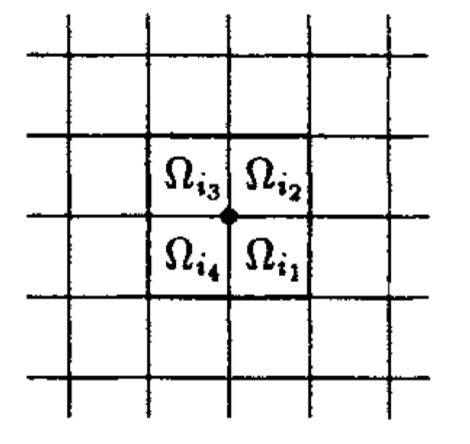
\includegraphics[width=3cm]{pavarino}
      \end{center}
      \begin{flushright}
        \textcite{Pavarino:1993} \hspace{4em}
      \end{flushright}
    \end{block}
  \end{onlyenv}

  \begin{onlyenv}<2>
    \begin{block}{Multigrid for nearly incompressible elasticity}
      The suggested smoother is block Jacobi smoother, which takes
      care of the kernel [...]. These kernel basis functions are
      captured by subspaces $V_{l,i}$ as shown
      \begin{center}
        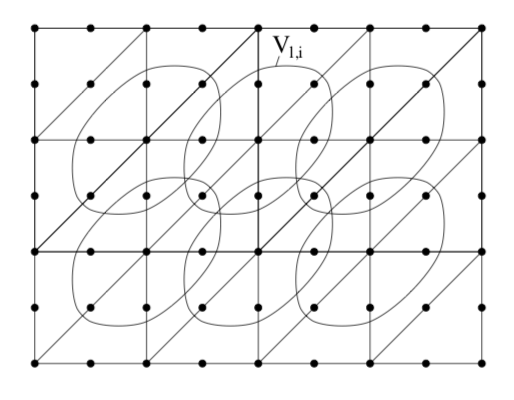
\includegraphics[height=3cm]{schoeberl}
      \end{center}
      \begin{flushright}
        \textcite{Schoeberl:1999} \hspace{4em}
      \end{flushright}
    \end{block}
  \end{onlyenv}

  \begin{onlyenv}<3>
    \begin{block}{Multigrid in $H(\div)$ and $H(\curl)$}
      To define the Schwarz smoothers, we can use a decomposition of
      $V_h$ into local patches consisting of all elements surrounding
      either an edge or a vertex.

      \begin{center}
        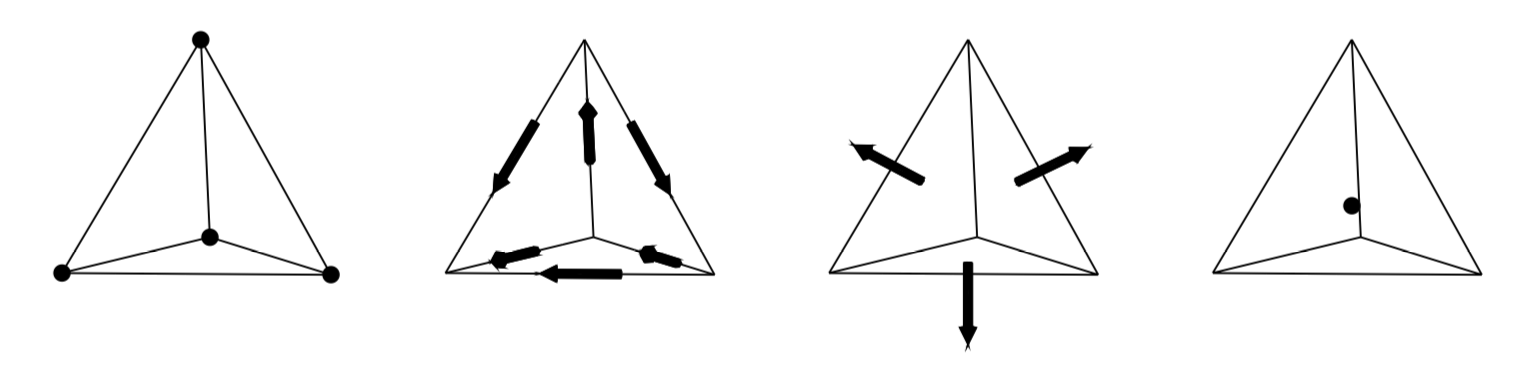
\includegraphics[height=2.5cm]{arnold}
      \end{center}
      \begin{flushright}
        \textcite{Arnold:2000} \hspace{4em}
      \end{flushright}
    \end{block}
  \end{onlyenv}

  \begin{onlyenv}<4>
    \begin{block}{An augmented Lagrangian approach to the Oseen problem}
      We use a block Gauss-Seidel method [...] based on the
      decomposition $V_h = \sum_{i=0}^l V_i$ [...For] P2-P0 finite
      elements the natural choice is to gather nodel DOFs for velocity
      inside ovals [around a vertex]

      \begin{center}
        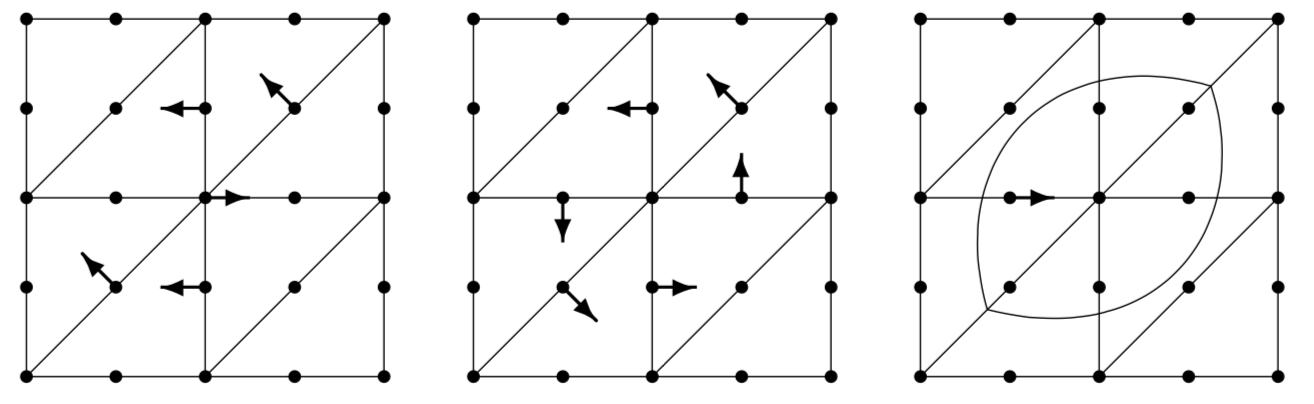
\includegraphics[height=2.5cm]{benzi}
      \end{center}
      \begin{flushright}
        \textcite{Benzi:2006} \hspace{4em}
      \end{flushright}
    \end{block}
  \end{onlyenv}
\end{frame}

\begin{frame}
  \frametitle{Unifying observation}

  \begin{block}{Abstract relaxation method}
    Choose a subspace decomposition
    \begin{equation*}
      V = \sum_i V_i
    \end{equation*}
    solve the problem on each subspace and combine the updates.
  \end{block}
  \begin{example}
    If $V_i$ is the span of a single basis function, then we have
    Jacobi or Gau\ss-Seidel relaxation (parallel or sequential
    subspace solves)
  \end{example}
  \begin{itemize}
  \item Decompose space (usually) based on some mesh decomposition
  \item Build and solve little problems on the resulting patches
  \item Combine additively or multiplicatively
  \end{itemize}
\end{frame}

\begin{frame}
  \frametitle{\texttt{PCPATCH}}
  \begin{block}{Topological decomposition}
    Use \texttt{DMPlex} to provide decomposition of mesh into patches.
  \end{block}

  \begin{block}{Space decomposition}
    Use topological decomposition plus \texttt{PetscSection} to
    determine degrees of freedom in each patch.
  \end{block}

  \begin{block}{Building patch problems}
    Callback interface to discretisation/PDE library.
  \end{block}
\end{frame}

\begin{frame}[fragile]
 \frametitle{Topological subspace definition via \texttt{DMPlex}}
 \begin{itemize}
 \item Each patch defined by set of mesh points (entities) on which the dofs
   we're going to solve for in the patch live
 \end{itemize}
 \begin{block}{Builtin}
   Specify patches by selecting:
   \begin{enumerate}
   \item Mesh points $\{p_i\}$ to iterate over (e.g.~vertices, cells)
   \item Adjacency relation that gathers points in patch
     \begin{itemize}
     \item[\texttt{star}] points in $\text{star}(p_i)$
     \item[\texttt{vanka}] points in $\text{closure}(\text{star}(p_i))$
     \end{itemize}
   \end{enumerate}
 \end{block}
 \begin{block}{User-defined}
   Callback provides \texttt{IS}es for each patch, plus iteration order.
\begin{minted}[fontsize=\scriptsize]{c}
 PetscErrorCode UserPatches(PC, PetscInt *npatch, IS **patches, 
                            IS *order, void *ctx);
\end{minted}
 \end{block}
\end{frame}

\begin{frame}
  \frametitle{Connect to dofs via \texttt{PetscSection}}
  \begin{itemize}
  \item Each patch defined by set of mesh points $\{p_i\}$
  \item Inspect \texttt{PetscSection} defining the function space
    layout to obtain global dof numbers
  \item These are the dofs we will solve for
    \begin{flushright}
      {\small wrinkle: for Vanka we also need to specify a constraint space.}
    \end{flushright}
  \item Create local renumbering on each patch (for local operator)
  \item Build scatters from global to patch vectors
  \item Finally, \emph{complete} patch using appropriate adjacency
    relationship (this pulls in dofs we need to see, but will not
    solve for)
  \end{itemize}
\end{frame}
\begin{frame}[fragile,t]
  \frametitle{Patch assembly}
  \begin{itemize}
  \item If we only want homogeneous Dirichlet, can use list of dofs to
    select from assembled global operator
  \item Other transmission conditions this doesn't work
  \item Instead, callback interface
  \item Naturally extends to \emph{nonlinear} smoothers
  \end{itemize}

  \begin{onlyenv}<1>
    \begin{block}{Callbacks}
\begin{minted}[fontsize=\scriptsize]{c}
 /* Patch Jacobian */
 UserComputeOp(PC, PetscInt point, Vec state, Mat op, IS cells, 
               PetscInt n, PetscInt *dofmap, void *ctx);
 /* Patch Residual */
 UserComputeF(PC, PetscInt point, Vec state, Vec f, IS cells, 
              PetscInt n, PetscInt *dofmapWithBcs, PetscInt *dofmap,
              void *ctx);
\end{minted}
    \end{block}
  \end{onlyenv}
  \begin{onlyenv}<2>
    \begin{block}{PDE library support}
      \begin{itemize}
      \item Works if you use \texttt{DMPlex} + \texttt{PetscDS}
\begin{minted}[fontsize=\scriptsize]{sh}
-pc_type patch
\end{minted}
      \item Works in Firedrake
\begin{minted}[fontsize=\scriptsize]{sh}
-pc_type python -pc_python_type firedrake.PatchPC
# Also
-snes_type python -snes_python_type firedrake.PatchSNES
\end{minted}
      \end{itemize}
    \end{block}
  \end{onlyenv}
\end{frame}

\section{Examples}

\begin{frame}
  \frametitle{What subspace to choose?}
  \begin{onlyenv}<1> Consider the problem: for
    $\alpha, \beta \in \mathbb{R}$, find $u \in V$ such that
    \begin{equation*}
      \alpha a(u, v) + \beta b(u, v) = (f, v) \quad \forall v \in V,
    \end{equation*}
    where $a$ is SPD, and $b$ is symmetric positive semidefinite.
  \end{onlyenv}
  \begin{theorem}[Sch\"oberl (1999); Lee, Wu, Xu, Zikatanov (2007)]
    Let the kernel be
    \begin{equation*}
      \mathcal{N} := \{ u \in V : b(u, v) = 0 \,\, \forall v \in V \}.
    \end{equation*}
    If the subspace decomposition \emph{captures the kernel}
    \begin{equation*}
      \mathcal{N} = \sum_i \mathcal{N} \cap V_i,
    \end{equation*}
    then convergence of the relaxation defined by this decomposition
    will be \emph{independent} of $\alpha$ and $\beta$.
    \nocite{Schoeberl:1999,Lee:2007}
  \end{theorem}
  \begin{onlyenv}<2>
    \begin{corollary}
      ``All'' we need to do is find a basis for the kernel.

      Appropriate discrete de Rham complexes can help.
    \end{corollary}
  \end{onlyenv}
\end{frame}

\begin{frame}[fragile]
  \frametitle{Nearly incompressible elasticity}
  \vspace*{-1.5\baselineskip}
  \begin{equation*}
    \text{Find $u \in V \subset H^1$ s.t.} \quad (\grad u, \grad v) + \gamma (\div u, \div v) = (f, v) \quad \forall v \in V.
  \end{equation*}
  \vspace*{-\baselineskip}
  \begin{block}{Stokes complex}
    \begin{equation*}
      \mathbb{R} \xrightarrow{\operatorname{id}} H^2 \xrightarrow{\grad} H^1(\curl)
      \xrightarrow{\curl} H^1 \xrightarrow{\div} L^2 \xrightarrow{\operatorname{null}} 0,
    \end{equation*}
    Decomposition must span $\ker \div = \range \curl$.

    Appropriate discrete spaces are constructed in \textcite{Neilan:2015a}: use
    star patch around vertices (with piecewise continuous space for
    $H^1$ of sufficiently high degree).
  \end{block}
  \begin{columns}
    \begin{column}{0.6\textwidth}
      \begin{onlyenv}<1>
\begin{minted}[fontsize=\scriptsize]{python}
{"ksp_type": "cg",
 "pc_type": "mg",
 "mg_levels": {
    "pc_type": "python",
    "pc_python_type": "firedrake.PatchPC",
    "patch": {


    }
 }
}
\end{minted}
      \end{onlyenv}
      \begin{onlyenv}<2>
\begin{minted}[fontsize=\scriptsize]{python}
{"ksp_type": "cg",
 "pc_type": "mg",
 "mg_levels": {
    "pc_type": "python",
    "pc_python_type": "firedrake.PatchPC",
    "patch": {
      "pc_patch_construct_dim": 0,

    }
 }
}
\end{minted}
      \end{onlyenv}
      \begin{onlyenv}<3->
\begin{minted}[fontsize=\scriptsize]{python}
{"ksp_type": "cg",
 "pc_type": "mg",
 "mg_levels": {
    "pc_type": "python",
    "pc_python_type": "firedrake.PatchPC",
    "patch": {
      "pc_patch_construct_dim": 0,
      "pc_patch_construct_type": "star",
    }
 }
}
\end{minted}
      \end{onlyenv}
    \end{column}
    \begin{column}{0.4\textwidth}
      \begin{center}
        \begin{tikzpicture}[scale=4]
          \tikzstyle{v}=[circle, fill, minimum size=0pt, inner sep=0pt]
          \tikzstyle{c}=[diamond, fill, minimum size=4pt, inner sep=0pt]
          \tikzstyle{e}=[rectangle, fill, minimum size=3pt, inner sep=0pt]
          \tikzstyle{select}=[draw, minimum size=3pt]
          \foreach \i/\k in {0/0, 0.25/1, 0.5/2, 0.75/3} {
            \foreach \j/\l in {0/0, 0.25/1, 0.5/2, 0.75/3} {
              \node[v] (v\k\l) at (\i, \j) {};
            }
          }

          \foreach \i in {0, 0.25, 0.5, 0.75} {
            \foreach \j/\k in {0/0.25, 0.25/0.5, 0.5/0.75} {
              \draw[thin, gray] (\i, \j) -- (\i, \k);
              \draw[thin, gray] (\j, \i) -- (\k, \i);
            }
          }
          \foreach \i/\j in {0/0.25, 0.25/0.5, 0.5/0.75} {
            \foreach \k/\l in {0/0.25, 0.25/0.5, 0.5/0.75} {
              \draw[thin, gray] (\i, \l) -- (\j, \k);
            }
          }

          \uncover<2->{
            \node[v, select] at (v11) {};
            \node[v, select] at (v21) {};
            \node[v, select] at (v12) {};
            \node[v, select] at (v22) {};
          }
          \foreach \a/\b in {0/1, 1/2, 2/3} {
            \foreach \c/\d in {1/0, 2/1, 3/2} {
              \node (c\a\c-\b\c-\b\d) at (barycentric cs:v\a\c=1,v\b\c=1,v\b\d=1) {};
              \node (c\a\d-\b\d-\a\c) at (barycentric cs:v\a\d=1,v\b\d=1,v\a\c=1) {};
            }
          }

          \uncover<3->{
            \draw[thick] \convexpath{
              c02-12-11,
              c11-21-12,
              c11-21-20,
              c10-20-11,
              c01-11-10,
              c01-11-02}{1pt};
            \draw[thick] \convexpath{
              c12-22-21,
              c21-31-22,
              c21-31-30,
              c20-30-21,
              c11-21-20,
              c11-21-12}{1pt};
            \draw[thick] \convexpath{
              c03-13-12,
 c12-22-13,
              c12-22-21,
              c11-21-12,
              c02-12-11,
              c02-12-03}{1pt};
            \draw[thick] \convexpath{
              c13-23-22,
              c22-32-23,
              c22-32-31,
              c21-31-22,
              c12-22-21,
              c12-22-13}{1pt};
          }
        \end{tikzpicture}
      \end{center}
    \end{column}
  \end{columns}
\end{frame}

\begin{frame}[fragile]
  \frametitle{H(div) Riesz map}
  \vspace{-1.5\baselineskip}
  \begin{equation*}
    \text{Find $u \in V \subset H(\div)$ s.t.}\quad (u, v) + \gamma (\div u, \div v) = (f, v) \quad \forall v \in V.
  \end{equation*}
  \vspace*{-\baselineskip}
  \begin{block}{Minimal continuity de Rham complex}
    \begin{equation*}
      \mathbb{R} \xrightarrow{\operatorname{id}} H^1 \xrightarrow{\grad} H(\curl)
      \xrightarrow{\curl} H(\div) \xrightarrow{\div} L^2 \xrightarrow{\operatorname{null}} 0,
    \end{equation*}
    Decomposition must span $\ker \div = \range \curl$.

    Choose $V$ to be a Raviart-Thomas space, the matching $H(\curl)$
    space has dofs on edges: use star patch around edges.
  \end{block}
  \begin{columns}
    \begin{column}{0.6\textwidth}
      \begin{onlyenv}<1>
\begin{minted}[fontsize=\scriptsize]{python}
{"ksp_type": "cg",
 "pc_type": "mg",
 "mg_levels": {
    "pc_type": "python",
    "pc_python_type": "firedrake.PatchPC",
    "patch": {


    }
 }
}
\end{minted}
      \end{onlyenv}
      \begin{onlyenv}<2>
\begin{minted}[fontsize=\scriptsize]{python}
{"ksp_type": "cg",
 "pc_type": "mg",
 "mg_levels": {
    "pc_type": "python",
    "pc_python_type": "firedrake.PatchPC",
    "patch": {
       "pc_patch_construct_dim": 1,

    }
 }
}
\end{minted}
      \end{onlyenv}
      \begin{onlyenv}<3->
\begin{minted}[fontsize=\scriptsize]{python}
{"ksp_type": "cg",
 "pc_type": "mg",
 "mg_levels": {
    "pc_type": "python",
    "pc_python_type": "firedrake.PatchPC",
    "patch": {
       "pc_patch_construct_dim": 1,
       "pc_patch_construct_type": "star",
    }
 }
}
\end{minted}
      \end{onlyenv}
    \end{column}
    \begin{column}{0.4\textwidth}
      \begin{center}
        \begin{tikzpicture}[scale=4]
          \tikzstyle{v}=[circle, fill, minimum size=0pt, inner sep=0pt]
          \tikzstyle{c}=[diamond, fill, minimum size=4pt, inner sep=0pt]
          \tikzstyle{e}=[rectangle, fill, minimum size=3pt, inner sep=0pt]
          \tikzstyle{select}=[draw, minimum size=3pt]
          \foreach \i/\k in {0/0, 0.25/1, 0.5/2, 0.75/3} {
            \foreach \j/\l in {0/0, 0.25/1, 0.5/2, 0.75/3} {
              \node[v] (v\k\l) at (\i, \j) {};
            }
          }

          \foreach \i in {0, 0.25, 0.5, 0.75} {
            \foreach \j/\k in {0/0.25, 0.25/0.5, 0.5/0.75} {
              \draw[thin, gray] (\i, \j) -- (\i, \k);
              \draw[thin, gray] (\j, \i) -- (\k, \i);
            }
          }
          \foreach \i/\j in {0/0.25, 0.25/0.5, 0.5/0.75} {
            \foreach \k/\l in {0/0.25, 0.25/0.5, 0.5/0.75} {
              \draw[thin, gray] (\i, \l) -- (\j, \k);
            }
          }
          \foreach \a/\b in {0/1, 1/2, 2/3} {
            \foreach \c/\d in {1/0, 2/1, 3/2} {
              \node (c\a\c-\b\c-\b\d) at (barycentric cs:v\a\c=1,v\b\c=1,v\b\d=1) {};
              \node (c\a\d-\b\d-\a\c) at (barycentric cs:v\a\d=1,v\b\d=1,v\a\c=1) {};
            }
          }
          \node (e1) at (barycentric cs:v12=1,v22=2) {};
          \node (e2) at (barycentric cs:v12=2,v22=1) {};

          \node (e3) at (barycentric cs:v11=1,v21=2) {};
          \node (e4) at (barycentric cs:v11=2,v21=1) {};

          \node (e5) at (barycentric cs:v21=1,v12=2) {};
          \node (e6) at (barycentric cs:v21=2,v12=1) {};

          \uncover<2->{
            \node[e, select] at (barycentric cs:v12=1,v22=1) {};
            \node[e, select] at (barycentric cs:v11=1,v21=1) {};
            \node[e, select] at (barycentric cs:v21=1,v12=1) {};
          }

          \uncover<3->{
            \draw[thick] \convexpath{
              c12-22-13,
              e1,
              c12-22-21,
              e2}{1pt};

            \draw[thick] \convexpath{
              c11-21-12,
              e3,
              c11-21-20,
              e4}{1pt};

            \draw[thick] \convexpath{
              c11-21-12,
              e5,
              c12-22-21,
              e6}{1pt};
          }
        \end{tikzpicture}
      \end{center}
    \end{column}
  \end{columns}

\end{frame}

\begin{frame}[fragile]
  \frametitle{H(curl) Riesz map}
  \vspace{-1.5\baselineskip}
  \begin{equation*}
    \text{  Find $u \in V \subset H(\curl)$ s.t.} \quad (u, v) + \gamma (\curl u, \curl v) = (f, v) \quad \forall v \in V.
  \end{equation*}
  \vspace{-\baselineskip}
  \begin{block}{Minimal continuity de Rham complex}
    \begin{equation*}
      \mathbb{R} \xrightarrow{\operatorname{id}} H^1 \xrightarrow{\grad} H(\curl)
      \xrightarrow{\curl} H(\div) \xrightarrow{\div} L^2 \xrightarrow{\operatorname{null}} 0,
    \end{equation*}
    Decomposition must span $\ker \curl = \range \grad$.

    Choose $V$ to be a N\'ed\'elec space, the matching $H^1$
    space has dofs at vertices: use star patch around vertices.
  \end{block}
  \begin{columns}
    \begin{column}{0.6\textwidth}
      \begin{onlyenv}<1>
\begin{minted}[fontsize=\scriptsize]{python}
{"ksp_type": "cg",
 "pc_type": "mg",
 "mg_levels": {
    "pc_type": "python",
    "pc_python_type": "firedrake.PatchPC",
    "patch": {


    }
 }
}
\end{minted}
      \end{onlyenv}
      \begin{onlyenv}<2>
\begin{minted}[fontsize=\scriptsize]{python}
{"ksp_type": "cg",
 "pc_type": "mg",
 "mg_levels": {
    "pc_type": "python",
    "pc_python_type": "firedrake.PatchPC",
    "patch": {
       "pc_patch_construct_dim": 0,

    }
 }
}
\end{minted}
      \end{onlyenv}
      \begin{onlyenv}<3->
\begin{minted}[fontsize=\scriptsize]{python}
{"ksp_type": "cg",
 "pc_type": "mg",
 "mg_levels": {
    "pc_type": "python",
    "pc_python_type": "firedrake.PatchPC",
    "patch": {
       "pc_patch_construct_dim": 0,
       "pc_patch_construct_type": "star",
    }
 }
}
\end{minted}
      \end{onlyenv}
    \end{column}
    \begin{column}{0.4\textwidth}
      \begin{center}
        \begin{tikzpicture}[scale=4]
          \tikzstyle{v}=[circle, fill, minimum size=0pt, inner sep=0pt]
          \tikzstyle{c}=[diamond, fill, minimum size=4pt, inner sep=0pt]
          \tikzstyle{e}=[rectangle, fill, minimum size=3pt, inner sep=0pt]
          \tikzstyle{select}=[draw, minimum size=3pt]
          \foreach \i/\k in {0/0, 0.25/1, 0.5/2, 0.75/3} {
            \foreach \j/\l in {0/0, 0.25/1, 0.5/2, 0.75/3} {
              \node[v] (v\k\l) at (\i, \j) {};
            }
          }

          \foreach \i in {0, 0.25, 0.5, 0.75} {
            \foreach \j/\k in {0/0.25, 0.25/0.5, 0.5/0.75} {
              \draw[thin, gray] (\i, \j) -- (\i, \k);
              \draw[thin, gray] (\j, \i) -- (\k, \i);
            }
          }
          \foreach \i/\j in {0/0.25, 0.25/0.5, 0.5/0.75} {
            \foreach \k/\l in {0/0.25, 0.25/0.5, 0.5/0.75} {
              \draw[thin, gray] (\i, \l) -- (\j, \k);
            }
          }

          \uncover<2->{
            \node[v, select] at (v11) {};
            \node[v, select] at (v21) {};
            \node[v, select] at (v12) {};
            \node[v, select] at (v22) {};
          }
          \foreach \a/\b in {0/1, 1/2, 2/3} {
            \foreach \c/\d in {1/0, 2/1, 3/2} {
              \node (c\a\c-\b\c-\b\d) at (barycentric cs:v\a\c=1,v\b\c=1,v\b\d=1) {};
              \node (c\a\d-\b\d-\a\c) at (barycentric cs:v\a\d=1,v\b\d=1,v\a\c=1) {};
            }
          }

          \uncover<3->{
            \draw[thick] \convexpath{
              c02-12-11,
              c11-21-12,
              c11-21-20,
              c10-20-11,
              c01-11-10,
              c01-11-02}{1pt};
            \draw[thick] \convexpath{
              c12-22-21,
              c21-31-22,
              c21-31-30,
              c20-30-21,
              c11-21-20,
              c11-21-12}{1pt};
            \draw[thick] \convexpath{
              c03-13-12,
              c12-22-13,
              c12-22-21,
              c11-21-12,
              c02-12-11,
              c02-12-03}{1pt};
            \draw[thick] \convexpath{
              c13-23-22,
              c22-32-23,
              c22-32-31,
              c21-31-22,
              c12-22-21,
              c12-22-13}{1pt};
          }
        \end{tikzpicture}
      \end{center}
    \end{column}
  \end{columns}
\end{frame}

\begin{frame}[fragile]
  \frametitle{Vanka for Stokes}
  Find $(u, p) \in V\times Q \subset (H^1)^d \times L^2$ s.t.
  \begin{equation*}
    (\grad u, \grad v) - (p, \div v) - (\div u, q) = (f, v) \quad \forall (v, q) \in V \times Q.
  \end{equation*}

  \begin{block}{Vanka patch}
    Solve simultaneously for $(u, p)$ on each pressure dof, gathering
    those velocity dofs that couple to the pressure dof.

    MAC: use patch around cells and gather closure

    Taylor-Hood: use patch around vertices and gather closure of star
    \nocite{Vanka:1986}
  \end{block}
  \pause
  \begin{columns}
    \begin{column}{0.5\textwidth}
      \begin{center}
        \begin{tikzpicture}[scale=4]
          \tikzstyle{v}=[circle, fill, minimum size=0pt, inner sep=0pt]
          \tikzstyle{c}=[diamond, fill, minimum size=4pt, inner sep=0pt]
          \tikzstyle{e}=[rectangle, fill, minimum size=3pt, inner sep=0pt]
          \tikzstyle{select}=[draw, minimum size=3pt]
          \foreach \i/\k in {0/0, 0.25/1, 0.5/2, 0.75/3} {
            \foreach \j/\l in {0/0, 0.25/1, 0.5/2, 0.75/3} {
              \node[v] (v\k\l) at (\i, \j) {};
            }
          }

          \foreach \i in {0, 0.25, 0.5, 0.75} {
            \foreach \j/\k in {0/0.25, 0.25/0.5, 0.5/0.75} {
              \draw[thin, gray] (\i, \j) -- (\i, \k);
              \draw[thin, gray] (\j, \i) -- (\k, \i);
            }
          }
          \foreach \i/\j in {0/0.25, 0.25/0.5, 0.5/0.75} {
            \foreach \k/\l in {0/0.25, 0.25/0.5, 0.5/0.75} {
              \draw[thin, gray] (\i, \l) -- (\j, \k);
            }
          }
          \foreach \a/\b in {0/1, 1/2, 2/3} {
            \foreach \c/\d in {1/0, 2/1, 3/2} {
              \node (c\a\c-\b\c-\b\d) at (barycentric cs:v\a\c=1,v\b\c=1,v\b\d=1) {};
              \node (c\a\d-\b\d-\a\c) at (barycentric cs:v\a\d=1,v\b\d=1,v\a\c=1) {};
            }
          }
          \node[c, select] at (c12-22-21) {};
          \node[c, select] at (c02-12-11) {};
          \node[c, select] at (c11-21-12) {};

          \draw[thick] \convexpath{v02,v12,v11}{1pt};
          \draw[thick] \convexpath{v12,v21,v11}{1pt};
          \draw[thick] \convexpath{v12,v22,v21}{1pt};
        \end{tikzpicture}
      \end{center}
    \end{column}
    \begin{column}{0.5\textwidth}
      \begin{center}
        \begin{tikzpicture}[scale=4]
          \tikzstyle{v}=[circle, fill, minimum size=0pt, inner sep=0pt]
          \tikzstyle{c}=[diamond, fill, minimum size=4pt, inner sep=0pt]
          \tikzstyle{e}=[rectangle, fill, minimum size=3pt, inner sep=0pt]
          \tikzstyle{select}=[draw, minimum size=3pt]
          \foreach \i/\k in {0/0, 0.25/1, 0.5/2, 0.75/3} {
            \foreach \j/\l in {0/0, 0.25/1, 0.5/2, 0.75/3} {
              \node[v] (v\k\l) at (\i, \j) {};
            }
          }

          \foreach \i in {0, 0.25, 0.5, 0.75} {
            \foreach \j/\k in {0/0.25, 0.25/0.5, 0.5/0.75} {
              \draw[thin, gray] (\i, \j) -- (\i, \k);
              \draw[thin, gray] (\j, \i) -- (\k, \i);
            }
          }
          \foreach \i/\j in {0/0.25, 0.25/0.5, 0.5/0.75} {
            \foreach \k/\l in {0/0.25, 0.25/0.5, 0.5/0.75} {
              \draw[thin, gray] (\i, \l) -- (\j, \k);
            }
          }
          \foreach \a/\b in {0/1, 1/2, 2/3} {
            \foreach \c/\d in {1/0, 2/1, 3/2} {
              \node (c\a\c-\b\c-\b\d) at (barycentric cs:v\a\c=1,v\b\c=1,v\b\d=1) {};
              \node (c\a\d-\b\d-\a\c) at (barycentric cs:v\a\d=1,v\b\d=1,v\a\c=1) {};
            }
          }
          \node[v, select] at (v12) {};
          \node[v, select] at (v21) {};

          \draw[thick] \convexpath{v03,v13,v22,v21,v11,v02}{1pt};
          \draw[thick] \convexpath{v12,v22,v31,v30,v20,v11}{1pt};
        \end{tikzpicture}
      \end{center}
    \end{column}
  \end{columns}
\end{frame}

\begin{frame}
  \frametitle{Nonlinear smoothers: \texttt{-snes\_type patch}}
  \begin{itemize}
  \item Algebraic splitting of assembled residuals and Jacobians
    \emph{tremendously} expensive
  \item Instead, take same approach with more callbacks
    \begin{itemize}
    \item Linearised operator
    \item and residual on a patch
    \end{itemize}
  \item Still quite expensive, but at least we don't have to assemble
    global problems on every patch
  \item Could improve with performance colouring
  \end{itemize}
\end{frame}

\begin{frame}[fragile]
  \frametitle{Example: Allen-Cahn}
  Find $\u \in V \subset H^1$ s.t.
  \begin{equation*}
    (\grad u, \grad v) - (f, v) + (u^3 - u, v) = 0 \quad \forall v
    \in V
  \end{equation*}
  \begin{columns}[T]
    \hspace{0.5em}
    \begin{column}{0.48\pagewidth}
      NJacobi
\begin{minted}[fontsize=\tiny]{python}
params = {
  "snes_type": "python",
  "snes_python_type": "firedrake.PatchSNES",
  "patch": {
    "snes_patch_partition_of_unity": False,
    "snes_patch_symmetrise_sweep": False,
    "snes_patch_local_type": "additive",
    "snes_patch_sub_mat_type": "seqdense",
    "snes_patch_construct_type": "star",
    "snes_patch_construct_dim": 0,
    "sub_snes_type": "newtonls",
    "sub_snes_linesearch_type": "basic",
    "sub_ksp_type": "preonly",
    "sub_pc_type": "lu",
  },
}
\end{minted}
    \end{column}
    \hspace{-0.5em}
    \begin{column}{0.48\pagewidth}
      NASM
\begin{minted}[fontsize=\tiny]{python}
params = {
  "snes_type": "python",
  "snes_python_type": "firedrake.PatchSNES",
  "patch": {
    "snes_patch_partition_of_unity": True,
    "snes_patch_symmetrise_sweep": False,
    "snes_patch_local_type": "additive",
    "snes_patch_sub_mat_type": "seqaij",
    "snes_patch_construct_type": "pardecomp",
    "snes_patch_pardecomp_overlap": 1,
    "sub_snes_type": "newtonls",
    "sub_snes_linesearch_type": "basic",
    "sub_ksp_type": "preonly",
    "sub_pc_type": "lu",
  },
}
\end{minted}
    \end{column}
  \end{columns}
\end{frame}
\begin{frame}
  \frametitle{Conclusions}
  \begin{itemize}
  \item Bidirectional solver/discretisation interface useful
  \item With topological decompositions in hand, can generically
    providing things that were previously by hand/from scratch
  \end{itemize}

  \begin{columns}[T]
    \begin{column}{0.47\pagewidth}
      \begin{block}{Future directions}
        \begin{itemize}
        \item Operators with face terms
        \item Other transmission conditions
        \item \dots concern that this starts to replicate full PDE
          library assembler
        \end{itemize}
      \end{block}
    \end{column}
    \pause
    \begin{column}{0.47\pagewidth}
      \begin{block}{Warts}
        \begin{itemize}
        \item Interface to callbacks is a bit finite elementy
        \item Ideally, each patch should be a \texttt{DM}
        \item Would enable ``big'' patches and fieldsplit/whatever,
          inside
        \item \dots is this too heavyweight to work for small patches?
        \end{itemize}
      \end{block}
    \end{column}
  \end{columns}
\end{frame}

\appendix
\begin{frame}
  \frametitle{References}
  \printbibliography[heading=none]
\end{frame}


\end{document}
